%Papers for top-Higgs Yukawa coupling, tth, and the analysis process: 
%https://arxiv.org/pdf/1807.02441.pdf
%http://cds.cern.ch/record/1690648/files/LCD_tth_note.pdf?version=1
%http://cds.cern.ch/record/1982243/files/CLICdp-Note-2015-001.pdf?version=1
%https://arxiv.org/pdf/1608.07538.pdf

\chapter{Physics studies for the Compact Linear Collider}
\label{chapter:analysis}

\epigraph{Somewhere, something incredible is waiting to be known.}{Carl Sagan}

This chapter will discuss the usage of full-scale detector simulations to assess the performance of the proposed \acrshort{CLIC}\textunderscore \acrshort{SiD} detector at the \acrlong{CLIC} machine, during the later stages where centre of mass energies in the tera-scale are possible.

This work was undertaken under the \acrfull{CLICdp} collaboration to determine the uncertainty on the measurement of the top-Higgs Yukawa coupling at the proposed \acrfull{CLIC} experiment at a centre-of-mass energy of $\sqrt{s}$ = 1.4 TeV, using the \acrshort{CLIC}\textunderscore \acrshort{SiD} detector concept. The analysis as discussed here focuses specifically on the hadronic channel, and when taken in combination with a similar analysis of the semi-leptonic channel performed by Yixuan Zhang\refthis allows the precision on the top-Higgs Yukawa coupling to be calculated.

These results were then contributed to a paper that summarised the top physics potential for \acrshort{CLIC} at $\sqrt{s}$ = 1.4 TeV, which was submitted to \acrshort{CERN}'s European Strategy Update in 2019. See references \cite{clic-top-quark-physics} \cite{clic-2018-summary}.

\section{Introduction}
One of the primary goals of all the future lepton colliders discussed in Chapter \ref{chapter:colliders} is to become ``Higgs factories'' -- machines that can produce large numbers of Higgs bosons in a variety of final states, allowing the Higgs sector of the \acrlong{SM} to be probed with unprecedented accuracy and coverage.

One of the best way to examine the Higgs sector is via the production of Higgs bosons in association with top quarks. The coupling between these two particles is the strongest Higgs coupling in the \acrshort{SM}, making it one of the easiest ways to examine the properties of the Higgs boson and the Higgs sector. This is the top-Higgs Yukawa coupling $y_t$. The \acrfull{SM} predicts the value of the top-Higgs Yukawa coupling to be:

\begin{equation}
	y_t^{SM} = \frac{\sqrt{2m_t}}{v}
\label{eq:yukawacoupling-sm-value}
\end{equation}

Many new models for new physics predict a deviation from the \acrshort{SM} value, e.g two Higgs-doublet models, the \acrfull{MSSM}, as well as composite Higgs or Little Higgs models. Determining the top-Higgs Yukawa coupling to the percent level is possible at future lepton colliders operating at energies in the tera-scale, due to the sensitivity of the tth cross-section. This will provide an important test of both the \acrlong{SM} and a multitude of these new physics models. 

In order to calculate the uncertainty on the Yukawa coupling, the uncertainty of the cross-section of the $e^+ e^- \rightarrow t\overline{t}h$ must first be calculated, and this can then be converted into the Yukawa coupling:

\begin{equation}
	\frac{\Delta y_t}{y_t} = \kappa \frac{\Delta \sigma}{\sigma}
\label{eq:crosssection-to-yukawa}
\end{equation}

Where $\sigma$ is the cross-section of the process, and $\kappa$ is some prefactor, normally assumed to be 0.5. This means that by determining the uncertainty on the cross-section of the tth process $\frac{\Delta \sigma}{\sigma}$, the uncertainty on the Yukawa coupling can be determined directly in a model-independent manner. 

%\begin{equation}
%	\frac{\Delta y_t}{y_t} = \kappa \frac{\sqrt{S+B}}{S} 
%\label{eq:signalbackground-to-yukawa}
%\end{equation}
%
%Where $S$ and $B$ are the number of signal events and background events selected in the final sample [...]

\section{The $e^+ e^- \rightarrow t\overline{t}h$ process}
The process best suited for studying the top-Higgs Yukawa coupling $y_t$ is the $e^+ e^- \rightarrow t\overline{t}h$ process, also referred to as the tth process. This is due to the direct interaction between the top quark and Higgs boson at the vertex.

% Ref for old BRs: http://pdg.lbl.gov/2013/listings/rpp2013-list-w-boson.pdf
The production of two top quarks in association with a Higgs makes this an ideal probe for this coupling. The top quark is only permitted to decay via the $t \rightarrow W^+ b $ process, but the decays of the W boson vary. W bosons can decay \textit{hadronically} into a pair of one up-type quark and one down-type quark (e.g. $u\overline{d}$ or $c\overline{s}$). Or they can decay \textit{leptonically} into a charged lepton and a neutrino of the same flavour (e.g. $e^- \overline{\nu}_e$ or $\mu^+ \nu_\mu$). The total branching ratio of all hadronic decays is 68\%, and the total branching ratio of all leptonic decays is 32\%. We denote a quark-antiquark pair as $q\overline{q}$, and a lepton-neutrino pair as $\ell \nu$.

Given that we focus only on events where the Higgs decays via the process $H \rightarrow b\overline{b}$, there are then three possible final states: %Redid these, double check once rendered
$$e^+ e^- \rightarrow t\overline{t}h \rightarrow q\overline{q}q\overline{q}b\overline{b}$$
$$e^+ e^- \rightarrow t\overline{t}h \rightarrow \ell \nu q \overline{q} b \overline{b}$$
$$e^+ e^- \rightarrow t\overline{t}h \rightarrow \ell \nu \ell \nu b \overline{b}$$

Due to the branching ratios, the hadronic and semi-leptonic final states are the most common, and the leptonic final state occurs less than ten percent of the time. This means that the most common final states all heavily rely upon jets, meaning that in order to perform accurate analysis of this process, jet energy resolution and jet reconstruction is of primary importance. As discussed in Chapter \ref{chapter:colliders}, the detector concepts for future lepton colliders are designed to focus on jet energy resolution and jet reconstruction, and utilise particle flow to augment this. \\

\begin{figure}[h]
	\centering
	\begin{tikzpicture}[line width=1.3 pt,scale=2]
		\draw[fermion]  (0,1) -- (1,0) ;
		\draw[fermionbar]  (0,-1) -- (1,0) ;
		\draw[vector]  (1,0) -- (2.5,0) ;
		\draw[fermion]  (2.5,0) -- (3.5,1) ;
		\draw[fermionbar]  (2.5,0) -- (3.5,-1) ;
		\draw[scalar]  (2.75,0.25) -- (3.5,0.) ;
		\node at (-0.3, 1) {$e^-$};
		\node at (-0.3, -1) {$e^+$};
		\node at (3.8, 1) {$t$};
		\node at (3.8, -1) {$\overline{t}$};
		\node at (3.8, 0) {$H$};
		\node at (1.75, 0.3) {$Z/\gamma *$};
	\end{tikzpicture} 
	\caption{Feynman diagram of the $tth$ event.}
	\label{figure:physics/SM/feynman-tth}
\end{figure}

There are significant irreducible backgrounds in the form of the $t\overline{t}Z$ and $t\overline{t}b\overline{b}$ processes, both of which are able to produce similar decays with 2, 4 or 6 leptons in the final state. These processes form a large contribution to the background due to their large cross-sections. The $t\overline{t}$ process is also a huge contribution to background because of its extremely high cross-section. 

Table \ref{table:physics/SM/generatedsamples} summarises the signal and background processes for this analysis.

\subsection{Higgstrahlung}
There is also another contribution to the tth final state in the form of \textit{higgstrahlung}. This process is actually an $e^+e^- \rightarrow t\overline{t}$ event where the intermediate $Z/\gamma *$ radiates a Higgs boson \textit{before} producing the $t\overline{t}$ pair (see Fig. \ref{figure:physics/SM/higgstrahlung}). This means the final state is tth but there is no vertex between the top quark and Higgs, meaning this process is not sensitive to the coupling. Therefore these events must be taken into account when calculating the total cross-section of the tth process when trying to determine the coupling. 

The effect of the higgstrahlung diagram is that the prefactor $\kappa$ from Equation \ref{eq:crosssection-to-yukawa} becomes greater than 0.5. The contribution from higgstrahlung is energy-dependent, and at low energies it is assumed to be negligible. However, for centre of mass ranges above 1 TeV, higgstrahlung contributes several percent or more of the tth events, and must be accounted for.

For this analysis, new work used NLO corrections to \acrshort{QCD}, the initial state radiation, and beamstahlung effects, to determine that $\kappa$ = 0.503 \cite{kappa-NLOQCD}. \\

\begin{figure}[h]
	\centering
	\begin{tikzpicture}[line width=1.3 pt,scale=2]
		\draw[fermion]  (0,1) -- (1,0) ;
		\draw[fermionbar]  (0,-1) -- (1,0) ;
		\draw[vector]  (1,0) -- (2.5,0) ;
		\draw[fermion]  (2.5,0) -- (3.5,1) ;
		\draw[fermionbar]  (2.5,0) -- (3.5,-1) ;
		\draw[scalar]  (1.75,0) -- (2.5,-1.) ;
		\node at (-0.3, 1) {$e^-$};
		\node at (-0.3, -1) {$e^+$};
		\node at (3.8, 1) {$t$};
		\node at (3.8, -1) {$\overline{t}$};
		\node at (2.8, -1) {$H$};
		\node at (1.75, 0.3) {$Z/\gamma *$};
	\end{tikzpicture} 
	\caption{Feynman diagram of the higgstrahlung process.}
	\label{figure:physics/SM/higgstrahlung}
\end{figure}

\begin{table}[htp]
\centering
	\begin{tabular}{ c l c r r }
	\hline \hline
	ProdID & Process & Cross-section (fb) & Sample weight & Events in 1.5 ab\textsuperscript{-1} \\ \hline \hline
	2435 & $t\overline{t}h$, 6 jets, $h \rightarrow b\overline{b}$ & 0.431 & 0.03 & 647 \\
	2441 & $t\overline{t}h$, 4 jets, $h \rightarrow b\overline{b}$ & 0.415 & 0.03 & 623 \\ \hline
	2429 & $t\overline{t}h$, 2 jets, $h \rightarrow b\overline{b}$ & 0.100 & 0.006 & 150 \\

	2438 & $t\overline{t}h$, 6 jets, $h \not\rightarrow b\overline{b}$ & 0.315 & 0.02 & 473	 \\
	2444 & $t\overline{t}h$, 4 jets, $h \not\rightarrow b\overline{b}$ & 0.303 & 0.02 & 455 \\
	2432 & $t\overline{t}h$, 2 jets, $h \not\rightarrow b\overline{b}$ & 0.073 & 0.004 & 110 \\

	2450 & $t\overline{t}Z$, 6 jets & 1.895 & 0.1 & 2843 \\
	2453 & $t\overline{t}Z$, 4 jets & 1.825 & 0.1 & 2738 \\
	2447 & $t\overline{t}Z$, 2 jets & 0.439 & 0.03 & 659 \\
	
	2423 & $t\overline{t}b\overline{b}$, 6 jets & 0.549 & 0.03 & 824 \\
	2426 & $t\overline{t}b\overline{b}$, 4 jets & 0.529 & 0.03 & 794 \\
	2420 & $t\overline{t}b\overline{b}$, 2 jets & 0.127 & 0.008 & 191 \\

	2417 & $t\overline{t}$ & 125.8 & 1.5 & 203700 \\ \hline

	\end{tabular}
	\caption{Table of all signal and background samples used for this analysis. The first two rows are the signal samples, the others are backgrounds.}
	\label{table:physics/SM/generatedsamples}
\end{table}

\section{Physics generation and samples}
The samples used for the study had been generated previously using ILCDIRAC\cite{ilc-dirac}. The physics generation was done predominantly in WHIZARD 1.95\cite{whizard}, using PYTHIA 6.422\cite{pythia} for the simulation of hadronisation and fragmentation. Due to constraints of WHIZARD, samples with final states with eight fermions were generated in \textsc{PhysSim}, also using PYTHIA. The mass of the Higgs boson was set at 125.0 GeV, and the mass of the top quark at 174.0 GeV. 

All samples were simulated at $\sqrt{s}$ = 1.4 TeV using unpolarised beams, assuming an integrated luminosity of 1.5 ab\textsuperscript{-1}. See Table \ref{table:physics/SM/generatedsamples} for a summary of all of the samples used. 

Following the generation of the underlying physics events, the interactions of the particles with the detector must be simulated. This was done using the \textsc{Geant4} toolkit\cite{geant4}, specifically the \textsc{Mokka} tool. Simulation of the signals that result from the interactions in the detector was done in \textsc{Marlin}\cite{marlin}.

At the end of this process, the Monte Carlo dataset is in a format identical to how information from the constructed detector would look. At this stage, the analysis can proceed as if the data were real. However, in addition to the simulated detector response, there is also the Monte Carlo truth information, which will allow correlation of the simulated detector response data with the ``true'' particles in the simulation itself. However, this is not used in this analysis.

\subsection{Detector model}
The samples for this study were simulated using the CLIC\textunderscore SiD detector model, built virtually within \textsc{Geant4}\cite{clic-sid-geant4}. This is the version of the \acrfull{SiD} as described in the \acrlong{CLIC} \acrfull{CDR}.

The CLIC\textunderscore SiD uses an all-silicon construction, with a design optimised for the needs of particle flow. It uses high-resolution vertex detectors and trackers, both based on silicon pixels and strips. The \acrshort{ECAL} and \acrshort{HCAL} use predominantly tungsten as the absorbing material, with steel used instead in the endcaps. These detectors are placed within a 5T solenoidal magnetic field, with an iron flux return yoke that is instrumented to act as a muon detector and tail catcher.

A more in-depth description of the \acrshort{SiD} detector concept can be found in Chapter \ref{chapter:colliders}.

\section{Event reconstruction}
The tth event has three possible final states, defined by the decay channel of the W bosons produced by the top quarks. The decay of a top quark will always produce a W boson and a bottom quark, while the W boson can decay one of two ways. Ignoring the decay of the Higgs boson, there are thus three possible combinations that can be seen in Table \ref{table:physics/final-states}. \\

\begin{table}[h]
\centering
	\begin{tabular}{ l c c c r }
	\hline \hline
	Decay Channel & Final State & No. of leptons & No. of jets & Branching Ratio \\ \hline \hline
	Fully hadronic & $q\overline{q}q\overline{q}b\overline{b}$ & 0 & 6 & 46\% \\ \hline
	Semi-leptonic &  $\ell \nu q\overline{q}b\overline{b}$ & 1 & 4 & 45\% \\ \hline
	Fully leptonic & $\ell \nu \ell \nu b\overline{b}$ & 2 & 2 & 9\% \\ \hline 
	\end{tabular}
	\caption{ }
	\label{table:physics/final-states}
\end{table}

Given the low branching ratio compared to the other channels, the fully leptonic state is not used in this analysis. Extended Feynman diagrams of the fully hadronic and semi-leptonic final states are shown in Figs. \ref{figure:physics/SM/feynman-tth-hadronic} and \ref{figure:physics/SM/feynman-tth-semileptonic}

\begin{figure}
	\centering
	\begin{tikzpicture}[line width=1.3 pt,scale=2.25]
		% Initial electrons	
		\draw[fermion]  (0,1) -- (1,0) ;
		\draw[fermionbar]  (0,-1) -- (1,0) ;
		% The central bar
		\draw[vector]  (1,0) -- (2.5,0) ;
		% The final top quarks
		\draw[fermion]  (2.5,0) -- (3.5,1) ;
		\draw[fermionbar]  (2.5,0) -- (3.5,-1) ;
		% The Higgs boson radiating off
		\draw[scalar]  (2.75,0.25) -- (3.5,0.) ;
		% The W+ and bottom quark coming off the top quark
		\draw[vector]  (3.5,1) -- (4.5,1.5) ;
		\draw[fermion]  (3.5,1) -- (4.5,0.5) ;
		% The W- and anti-bottom quark coming off the anti-top quark
		\draw[fermionbar]  (3.5,-1) -- (4.5,-0.5) ;
		\draw[vector]  (3.5,-1) -- (4.5,-1.5) ;
		% The quark-antiquark pair coming off the W+
		\draw[fermion]  (4.5, 1.5) -- (5.5,2) ;
		\draw[fermion]  (4.5, 1.5) -- (5.5,1) ;
		% The quark-antiquark pair coming off the W-
		\draw[fermionbar]  (4.5, -1.5) -- (5.5,-1) ;
		\draw[fermionbar]  (4.5, -1.5) -- (5.5,-2) ;
		% Labels
		\node at (-0.3, 1) {$e^-$};
		\node at (-0.3, -1) {$e^+$};
		\node at (3.8, 1) {$t$};
		\node at (3.8, -1) {$\overline{t}$};
		\node at (3.8, 0) {$H^0$};
		\node at (5.0, 1.5) {$W^+$};
		\node at (4.8, 0.5) {$b$};
		\node at (4.8, -0.5) {$\overline{b}$};
		\node at (5.0, -1.5) {$W^-$};
		\node at (5.8,2) {$q$};
		\node at (5.8,1) {$\overline{q}$};
		\node at (5.8,-1) {$q$};
		\node at (5.8,-2) {$\overline{q}$};
	\end{tikzpicture} 
	\caption{Extended Feynman diagram of the tth event, showing the fully-hadronic decay channel with the final state $q\overline{q}q\overline{q}b\overline{b}$. \newline}
	\label{figure:physics/SM/feynman-tth-hadronic}
	\begin{tikzpicture}[line width=1.3 pt,scale=2.25]
		% Initial electrons
		\draw[fermion]  (0,1) -- (1,0) ;
		\draw[fermionbar]  (0,-1) -- (1,0) ;
		% The central bar
		\draw[vector]  (1,0) -- (2.5,0) ;
		% The final top quarks
		\draw[fermion]  (2.5,0) -- (3.5,1) ;
		\draw[fermionbar]  (2.5,0) -- (3.5,-1) ;
		% The Higgs boson radiating off
		\draw[scalar]  (2.75,0.25) -- (3.5,0.) ;
		% The W+ and bottom quark coming off the top quark
		\draw[vector]  (3.5,1) -- (4.5,1.5) ;
		\draw[fermion]  (3.5,1) -- (4.5,0.5) ;
		% The W- and anti-bottom quark coming off the anti-top quark
		\draw[fermionbar]  (3.5,-1) -- (4.5,-0.5) ;
		\draw[vector]  (3.5,-1) -- (4.5,-1.5) ;
		% The lepton-neutrino pair coming off the W+
		\draw[fermion]  (4.5, 1.5) -- (5.5,2) ;
		\draw[fermion]  (4.5, 1.5) -- (5.5,1) ;
		% The quark-antiquark pair coming off the W-
		\draw[fermionbar]  (4.5, -1.5) -- (5.5,-1) ;
		\draw[fermionbar]  (4.5, -1.5) -- (5.5,-2) ;
		% Labels
		\node at (-0.3, 1) {$e^-$};
		\node at (-0.3, -1) {$e^+$};
		\node at (3.8, 1) {$t$};
		\node at (3.8, -1) {$\overline{t}$};
		\node at (3.8, 0) {$H^0$};
		\node at (5.0, 1.5) {$W^+$};
		\node at (4.8, 0.5) {$b$};
		\node at (4.8, -0.5) {$\overline{b}$};
		\node at (5.0, -1.5) {$W^-$};
		\node at (5.8,2) {$\ell$};
		\node at (5.8,1) {$\nu$};
		\node at (5.8,-1) {$q$};
		\node at (5.8,-2) {$\overline{q}$};
	\end{tikzpicture} 
	\caption{Extended Feynman diagram of the tth event, showing the semi-leptonic decay channel  with the final state $\ell\nu q\overline{q}b\overline{b}$.}
	\label{figure:physics/SM/feynman-tth-semileptonic}
\end{figure}

\subsection{Lepton identification}
The first step of the analysis procedure is to distinguish between the hadronic and semi-leptonic final states. This is done by finding isolated leptons in the final state. If there are no final-state leptons it is classified as a hadronic event; if there is a single lepton in the final state it is classified as a semi-leptonic event. If there are two leptons in the final state it is classified as a leptonic event and discarded.

Finding the leptons that have been produced by the decay of the W boson is relatively simple, as leptons produced in this decay have a much higher energy than leptons produced in jets. In general, these leptons have energies in the 50-350 GeV range, which can be found from the reconstructed track energy. However there are additional properties of these leptons that can be used to improve their selection.

\begin{figure}[h]
	\centering
	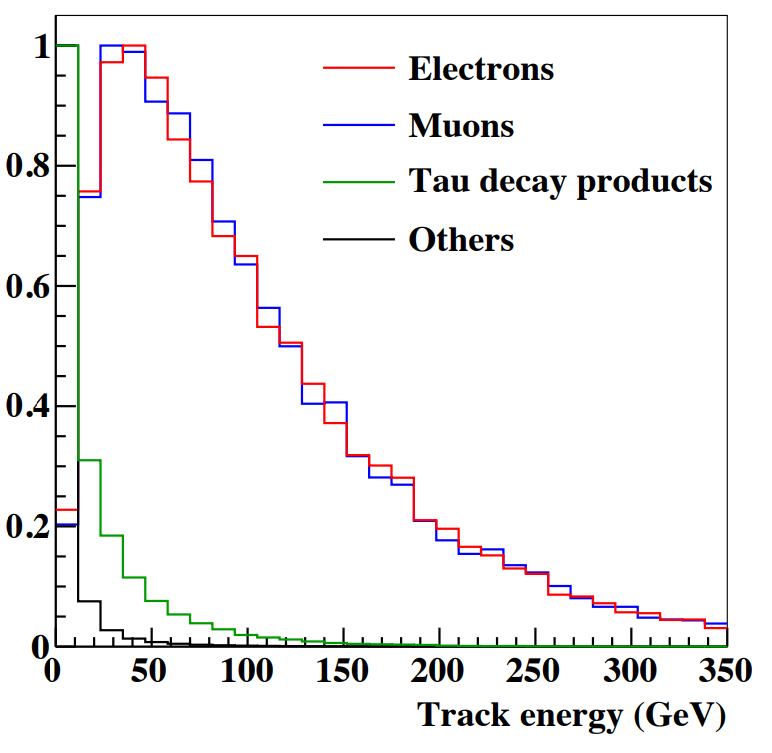
\includegraphics[width=0.55\textwidth]{../Pictures/Analysis/track-energy.png}
	\caption{Plots of the track energy for truth-matched reconstructed electrons, muons and tau decay products, and all other reconstructed particles that were not truth-matched to a lepton.}
	\label{figure:analysis/leptons/track-energy}
\end{figure}

Leptons produced within jets will detected within the same region as the other particles from the same jet, in a high-occupancy region of the detector. Therefore, an isolated lepton detected in a low-occupancy region of the detector is more likely to have originated from the decay of a W boson, rather than from a jet.

The impact parameter (\acrshort{IP-analysis}) is the distance between the primary vertex that produced a particle, and the closest approach of the particle's track. Electrons and muons produced from W boson decays have much lower \acrshort{IP-analysis}s than other particles or tau decay products. The impact parameter can be considered in either the longitudinal ($Z_0$) or radial ($d_0$) components, which can be combined for a 3D \acrshort{IP-analysis}:

\begin{equation}
	\centering
	R_0 = \sqrt{Z_0^2 + d_0^2}
\label{eq:impact-parameter}
\end{equation}

\begin{figure}[p]
	\centering
	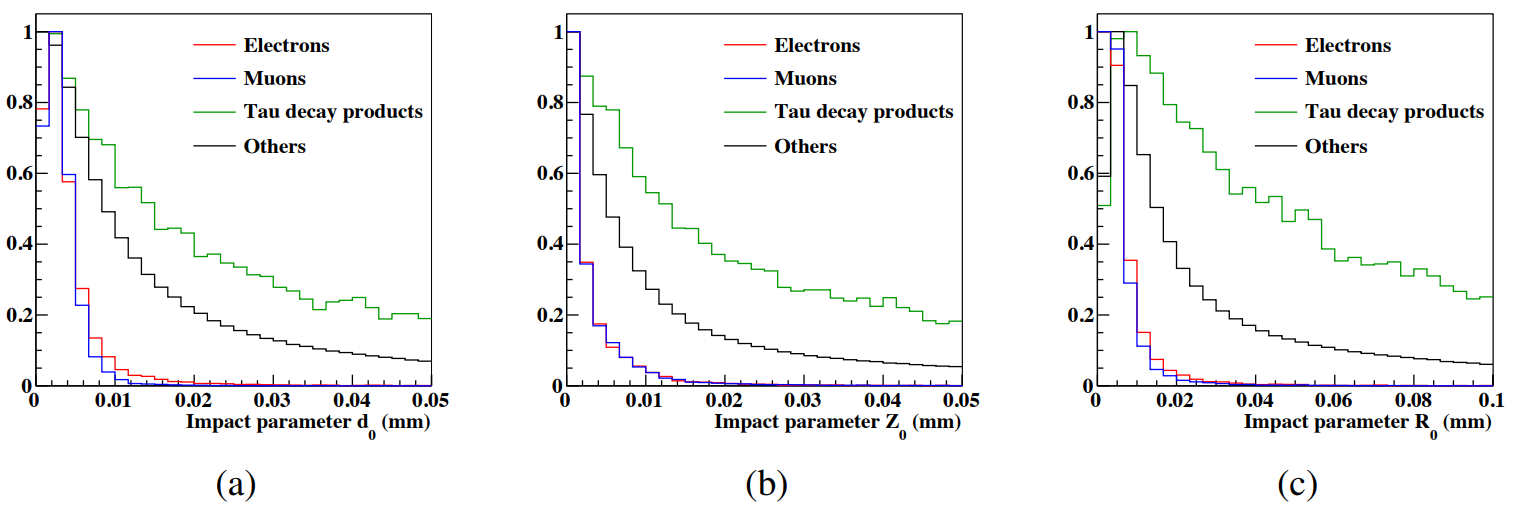
\includegraphics[width=0.95\textwidth]{../Pictures/Analysis/impact-parameter.png}
	\caption{Plots of the impact parameters $d_0$, $Z_0$, and $R_0$ for truth-matched reconstructed electrons, muons and tau decay products, and all other reconstructed particles that were not truth-matched to a lepton.}
	\label{figure:analysis/leptons/impact-parameter}
\end{figure}

Another property useful for distinguishing electrons and muons decaying from W bosons is the profile of their energy deposition in the calorimeters. We can define a ratio of the energy deposited in the electromagnetic calorimeter to the total energy deposited in the calorimeters:

\begin{equation}
	R_{CAL} = \frac{E_{CAL}}{E_{ECAL} + E_{HCAL}}
\label{eq:calorimeter-ratio}
\end{equation}

Since electrons are contained within the \acrshort{ECAL}, their value of $R_{CAL}$ will peak at 1. Muons deposit their energy throughout both calorimeters, so will peak at approximately 0.2. Taus cannot be identified this way, as their decay products do not deposit predictable amounts of energy in the calorimeters.

\begin{figure}[p]
	\centering
	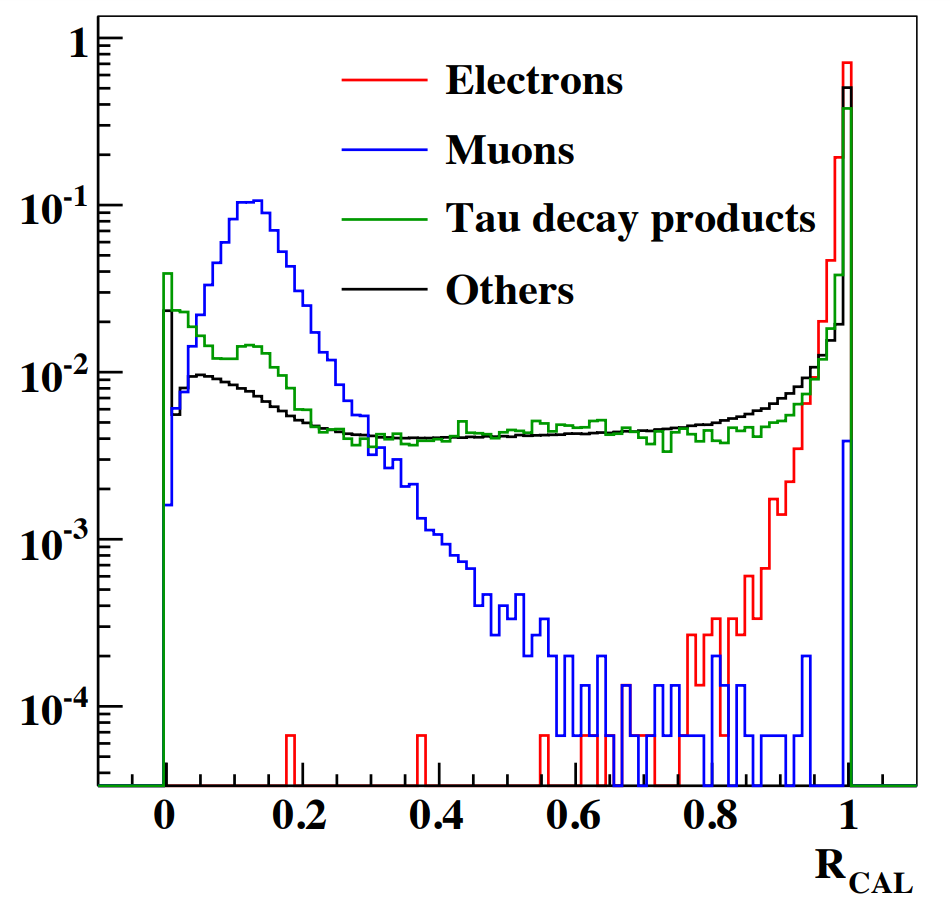
\includegraphics[width=0.55\textwidth]{../Pictures/Analysis/cal-energy.png}
	\caption{Plot of the calorimeter energy ratio $R_{CAL}$ for truth-matched reconstructed electrons, muons and tau decay products, and all other reconstructed particles that were not truth-matched to a lepton. Electrons and muons from W boson decays can be clearly distinguished from each other, and from  other particles.}
	\label{figure:analysis/leptons/cal-energy}
\end{figure}

\subsubsection{IsolatedLeptonFinder}
To perform the selections to find isolated leptons, the \texttt{IsolatedLeptonFinder} processor within \textsc{Marlin} was used. This lepton finder processor uses criteria based on the properties described above to identify isolated leptons:

\begin{itemize}
	\item Track energy greater than 15 GeV
	\item Each of $d_0$, $Z_0$ and $R_0$ greater than 0.05 mm
	\item $R_{CAL}$ greater than 0.5, or in the range 0.05-0.3	
\end{itemize}

The first cut on track energy already retains 96.5\% of the reconstructed electrons and muons, while accepting only 9.6\% of other particles. With the additional criteria, this becomes 87.3\% isolated leptons and 0.4\% other particles.

\subsection{Tau identification}
Taus cannot be identified directly due their extremely short lifetime ($2.9 \times 10^{-13}$s), and must instead be identified from their decay products, which can vary significantly. Taus most commonly decay hadronically into a number of charged or neutral pions, or leptonically into a lepton-neutrino pair; in each case always also producing an undetectable tau neutrino. 

Identification of taus was done using the \texttt{TauFinder} processor\cite{taufinder} within \textsc{Marlin}, which was adapted for this analysis. The criteria were determined using truth-matching the simulation data to find the best strategy to identify taus.

The processor looks at particles that may have decayed from taus, and forms a tau candidate based on their properties. First it creates a seed track with a $p_T$ greater than 10 GeV, adding all particles within a 0.04 rad cone of the seed track to the tau candidate if every particle has $p_T >$ 2 GeV and $R_0$ within the range 0.01-0.05mm. The reconstructed tau candidate must then be formed of an odd number of charged tracks, with an invariant mass of less than 1.5 GeV. This mass is slightly lower than the true tau invariant mass to account for missing energy in the form of the tau neutrinos. Then an isolation ring is defined in the region 0.04-0.24 rad around the tau candidate seed track. In order to be considered a tau, there must be fewer than five particles in the isolation ring, with a total energy of less than 5 GeV.

\subsection{Reconstruction of Higgs, top and W boson candidates}
Before jet clustering, any isolated leptons are removed from the event. The event is then clustered using the $k_t$ algorithm with $R = 1.0$. The jet clustering algorithm is run in exclusive mode, forcing the event into a specific number of jets -- in  the case of the hadronic analysis, eight jets. Once this is complete, the jet particles are then reclustered using the Durham algorithm .

Following this, the properties of the jets are used to reconstruct candidates for the Higgs boson, top quarks, and W bosons. This is done by doing a calculation of the invariant masses of the tops, W bosons, and Higgs, resulting in a $\chi^2$ value. By computing this $\chi^2$ value for all possible combinations of jets and finding the combination that results in the minimum, the jets can be matched to which particles produced them. 

\begin{equation}
  \centering
	\chi^2 = \frac{(m_{12} - m_W)^2}{\sigma^2_W} + \frac{(m_{123} - m_t)^2}{\sigma^2_{t}} + \frac{(m_{45} - m_W)^2}{\sigma^2_W} + \frac{(m_{456} - m_t)^2}{\sigma^2_{t}} + \frac{(m_{78} - m_H)^2}{\sigma^2_H}
\label{eq:chi-square}
\end{equation}

where the numbered subscripts indicate the indices of the jets used to form the invariant masses $m$. A similar equation is used for the semi-leptonic channel, using only the 6 jets present in that process. The $\chi^2$ values are extremely useful for selection, as events that are not tth, or are tth events without the fully hadronic decay channel, will have poor $\chi^2$ values, as the jets the event was forced into do not represent physical jets.

\subsection{Flavour tagging}
The majority of the backgrounds for this analysis do not have four b-jets in the final state. Therefore reliable b-tagging is an important source of discriminating power.

For this analysis, b-tagging is done in the LCFIPlus package \cite{lcfiplus}, using simulated samples of $e^+ e^- \rightarrow qqqqqq$ where all quarks have the same flavour. The high number of jets in the final state means that the kinematic properties of the jets are similar to those in the analysis samples. Four \acrfull{BDT} are trained for b-tagging, and four for c-tagging, trained using the properties of the jets. These \acrshort{BDT}s then give b-tag and c-tag probabilities for each jet, which are used for event selection in the next step.

\section{Event selection}
The final event selection is done using \acrfull{BDT}, implemented in the \acrfull{TMVA}. The \acrshort{BDT}s for the hadronic channel are trained separately to the semi-leptonic channel. No pre-selection is used in this analysis. For the hadronic channel, the following variables are used:

\begin{itemize}
	\item Reconstructed Higgs mass
	\item Number of reconstructed particles in the event
	\item Visible jet energy
	\item Missing transverse momentum ($p_T$)
	\item $\chi^2$ of the jet grouping
	\item Event shape variables -- thrust, sphericity, aplanarity
	\item Four highest b-tag values and their corresponding c-tags
	\item The cosine of the decay angle of the $h \rightarrow b\overline{b}$, and the cosine of the angles between the Higgs and each top quark
	\item The distance between the two closest jets, as defined by the Durham jet clustering algorithm
	\item The energy of the four lowest-energy jets
	\item The cosine of the angle of the two jets closest to the beam-axis
\end{itemize}

The \acrshort{BDT}s use the sample split into two randomly. The first half is used for training the \acrshort{BDT}s, and the other becomes the samples used by the \acrshort{BDT}.

The BDTs then produce a BDT response value, and a value for this is chosen to optimise the event selection. The criteria for an optimal event selection is the maximal significance:

\begin{equation}
	\frac{S}{\sqrt{S + B}}
\label{eq:significance}
\end{equation}

Where $S$ is the number of signal events selected, and $B$ is the number of background events selected. This results in a significance of 10.44 for the fully hadronic channel.

The result of of applying the selection to the BDT response on the event samples can be seen in Table \ref{table:physics/SM/selections}.

\begin{table}[ht]
\centering
	\begin{tabular}{ l r r r }
	\hline \hline
	Process & $N$ & fully hadronic & semi-leptonic \\ \hline \hline
	$t\overline{t}h$, 6 jets, $h \rightarrow b\overline{b}$ & 647 & 367 & 38 \\
	$t\overline{t}h$, 4 jets, $h \rightarrow b\overline{b}$ & 623 & 1 & 270 \\ \hline
	$t\overline{t}h$, 2 jets, $h \rightarrow b\overline{b}$ & 150 & 2 & 22 \\

	$t\overline{t}h$, 6 jets, $h \not\rightarrow b\overline{b}$ & 473 & 54 & 11	 \\
	$t\overline{t}h$, 4 jets, $h \not\rightarrow b\overline{b}$ & 455 & 8 & 22\\
	$t\overline{t}h$, 2 jets, $h \not\rightarrow b\overline{b}$ & 110 & 0 & 1 \\

	$t\overline{t}Z$, 6 jets & 2843 & 345 & 34 \\
	$t\overline{t}Z$, 4 jets & 2738 & 59 & 217 \\
	$t\overline{t}Z$, 2 jets & 659 & 1 & 16 \\
	
	$t\overline{t}b\overline{b}$, 6 jets & 824 & 326 & 26 \\
	$t\overline{t}b\overline{b}$, 4 jets & 794 & 57 & 226 \\
	$t\overline{t}b\overline{b}$, 2 jets & 191 & 2 & 18 \\

	$t\overline{t}$ & 203700 & 498 & 742 \\ \hline

	total $t\overline{t}H$ signal & 2458 & 433 (17.6\%) & 365 (14.8\%) \\ 
	total background & 211749 & 1287 (0.61\%) & 1280 (0.60\%) \\
	Significance &   & 10.44 & 9.00 \\ \hline

	\end{tabular}
	\caption{Expected numbers of signal and background events classified by the \acrshort{BDT}s as either fully hadronic or semi-leptonic in 1.5 ab\textsuperscript{-1} at $\sqrt{s}$ = 1.4 TeV.}
	\label{table:physics/SM/selections}
\end{table}

\section{Results}
In order to extract the top-Higgs Yukawa coupling $y_t$, the total cross-section of the tth process must be calculated. Using  the output of the \acrshort{BDT}s, the precision on the cross-section of the tth process using just the hadronic channel is 9.6\%. A similar analysis by Yixuan Zhang found the precision for the semi-leptonic channel to be 11.1\%. Thus the combined uncertainty for the cross-section of both decay channels is:

$$\Delta\sigma = 7.30\% $$

When extracting the top-Higgs Yukawa coupling $y_t$ from the total cross-section, the contribution of the higgstrahlung diagram (Fig. \ref{figure:physics/SM/higgstrahlung}) must be taken into account, as this is a tth final state that has no vertex between the top and the Higgs and thus is not sensitive to the coupling.

Thus the uncertainty on the top-Higgs Yukawa coupling is:

$$\frac{\Delta g_{tth}}{g_{tth}} = 0.503 \frac{\Delta\sigma(t\overline{t}H)}{\sigma(t\overline{t}H)} = 3.86\% $$


\begin{figure}[h]
	\centering
	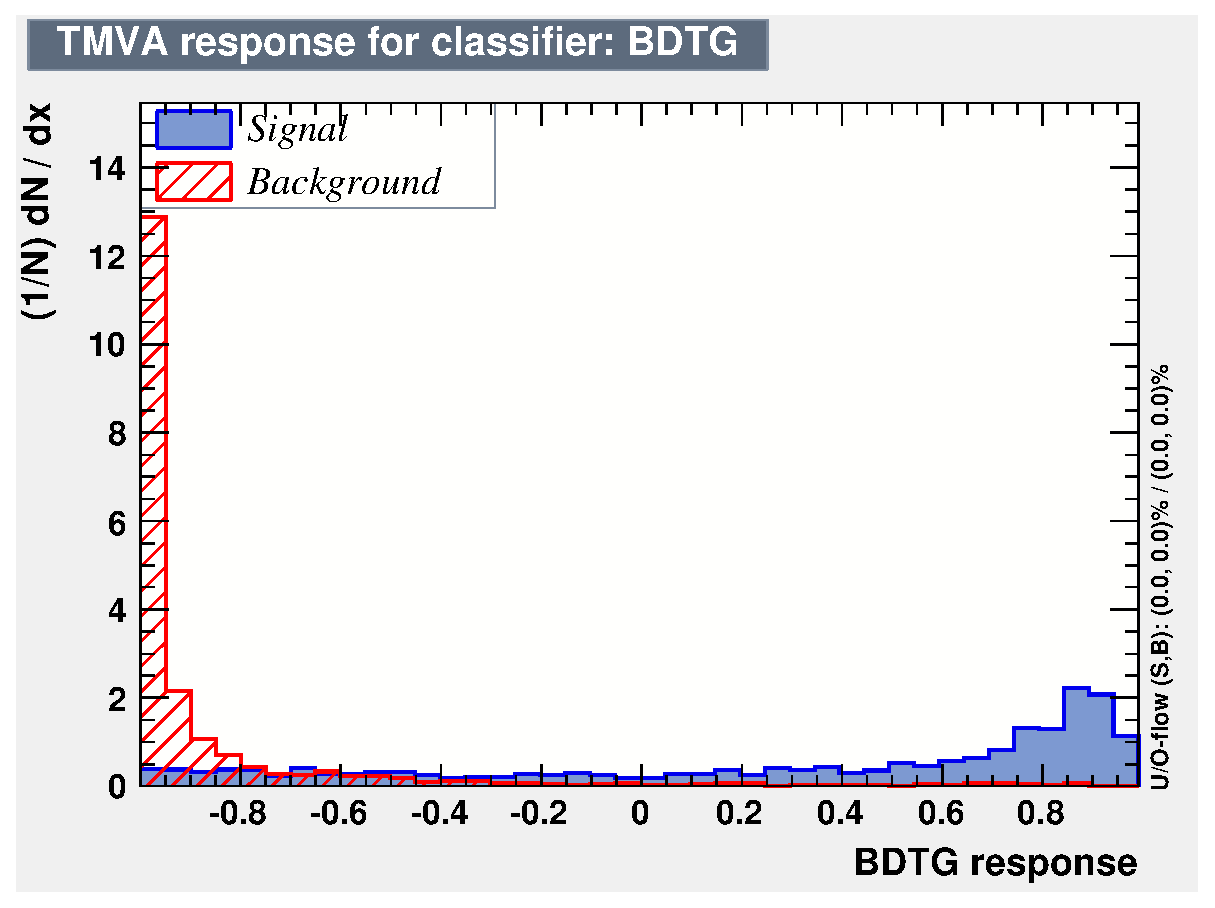
\includegraphics[width=0.55\textwidth]{../Pictures/Analysis/BDTs/mva_BDTG.eps}
	\caption{Normalised BDTG response for signal and background.}
	\label{figure:analysis/results/bdt-response-sb}
\end{figure}

\begin{figure}[h]
	\centering
	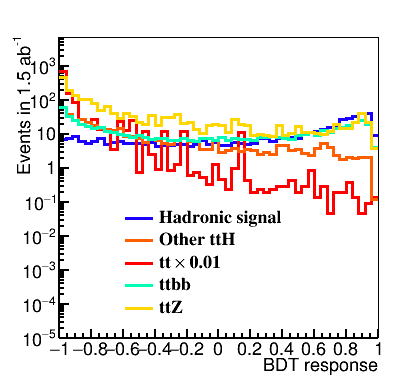
\includegraphics[width=0.55\textwidth]{../Pictures/Analysis/BDTs/MVA_BDTG_comb_had.png}
	\caption{BDTG scaled to the number of events expected in 1.5 ab\textsuperscript{-1}.}
	\label{figure:analysis/results/bdt-response-combined}
\end{figure}

\begin{figure}[h]
	\centering
	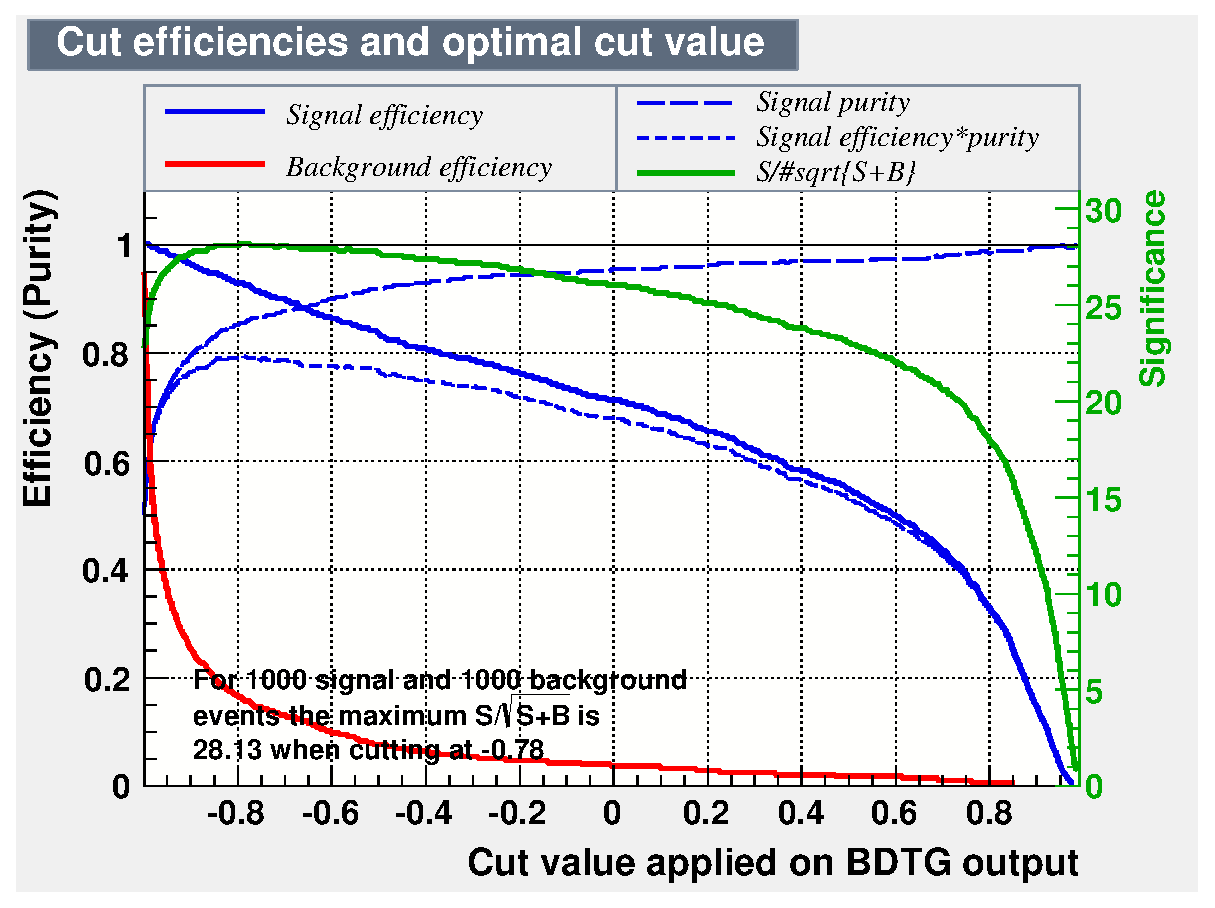
\includegraphics[width=0.55\textwidth]{../Pictures/Analysis/BDTs/mvaeffs_BDTG.eps}
	\caption{Signal and background efficiencies for different values of the cut valued applied on the results of the BDTs.}
	\label{figure:analysis/results/tmva-efficiency}
\end{figure}

\begin{figure}[h]
	\centering
	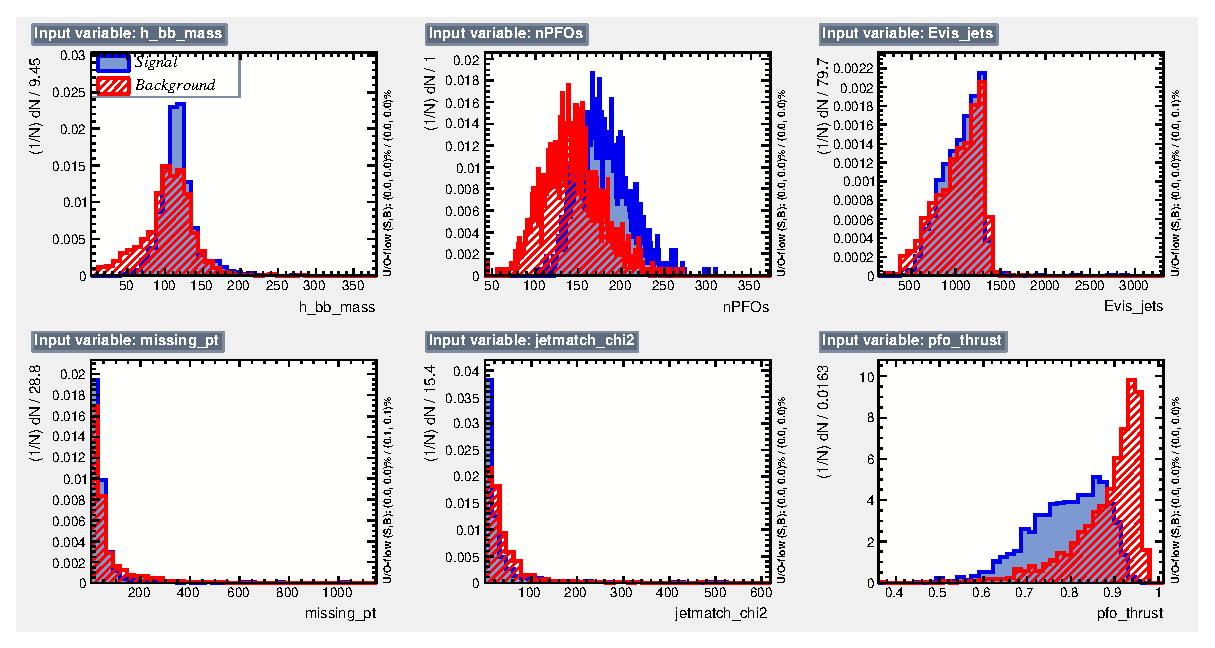
\includegraphics[width=0.95\textwidth]{../Pictures/Analysis/BDTs/variables_id_c1.eps}
	\caption{Input variables for the BDTs: Higgs mass from $b\overline{b}$ jets; number of particle flow objects; visible jet energy; missing transverse momentum; $\chi^2$ value from jets (Eq. \ref{eq:chi-square}); event thrust.}
	\label{figure:analysis/results/tmva-inputs-1}
\end{figure}

\begin{figure}[h]
	\centering
	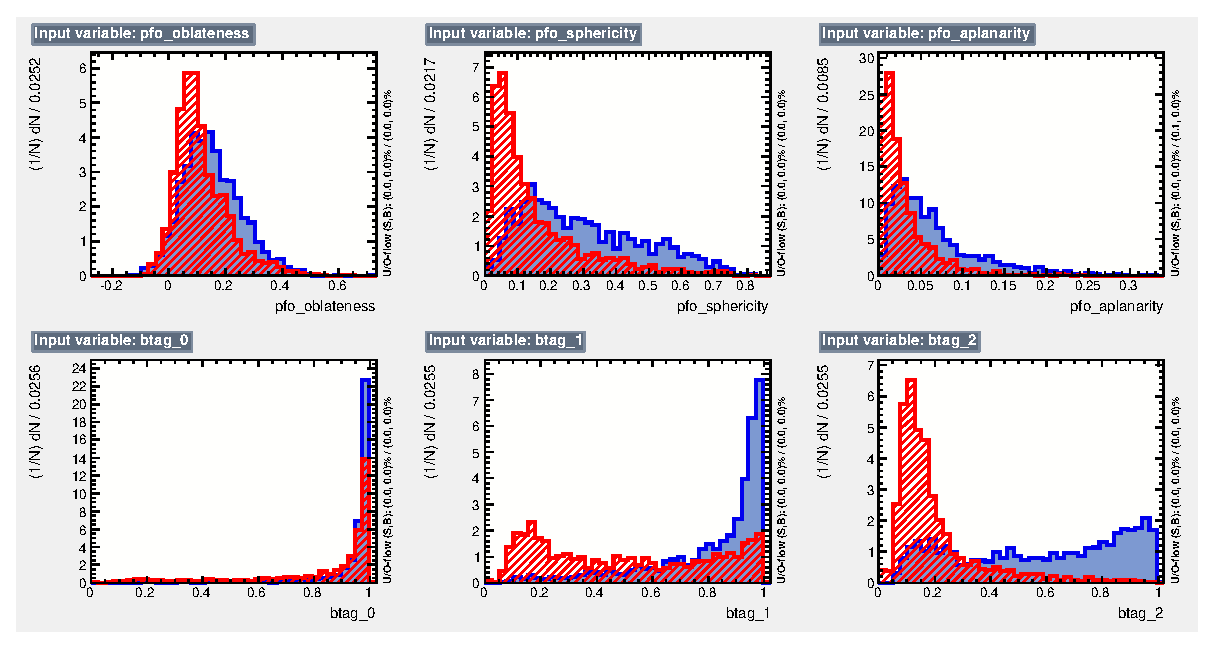
\includegraphics[width=0.95\textwidth]{../Pictures/Analysis/BDTs/variables_id_c2.eps}
	\caption{Input variables for the BDTs: event oblateness; event sphericity; event aplanarity; first, second and third highest b-tags.}
	\label{figure:analysis/results/tmva-inputs-2}
\end{figure}

\begin{figure}[h]
	\centering
	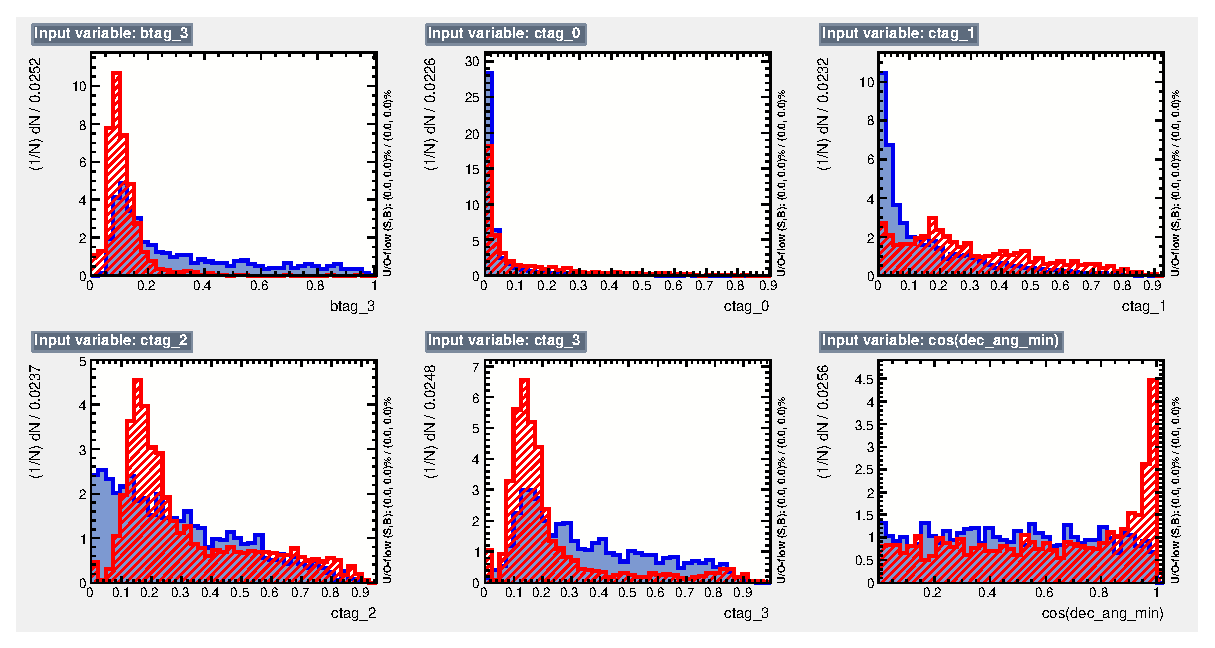
\includegraphics[width=0.95\textwidth]{../Pictures/Analysis/BDTs/variables_id_c3.eps}
	\caption{Input variables for the BDTs: four highest b-tag; first, second, third and fourth highest c-tags; [cos].}
	\label{figure:analysis/results/tmva-inputs-3}
\end{figure}

\begin{figure}[h]
	\centering
	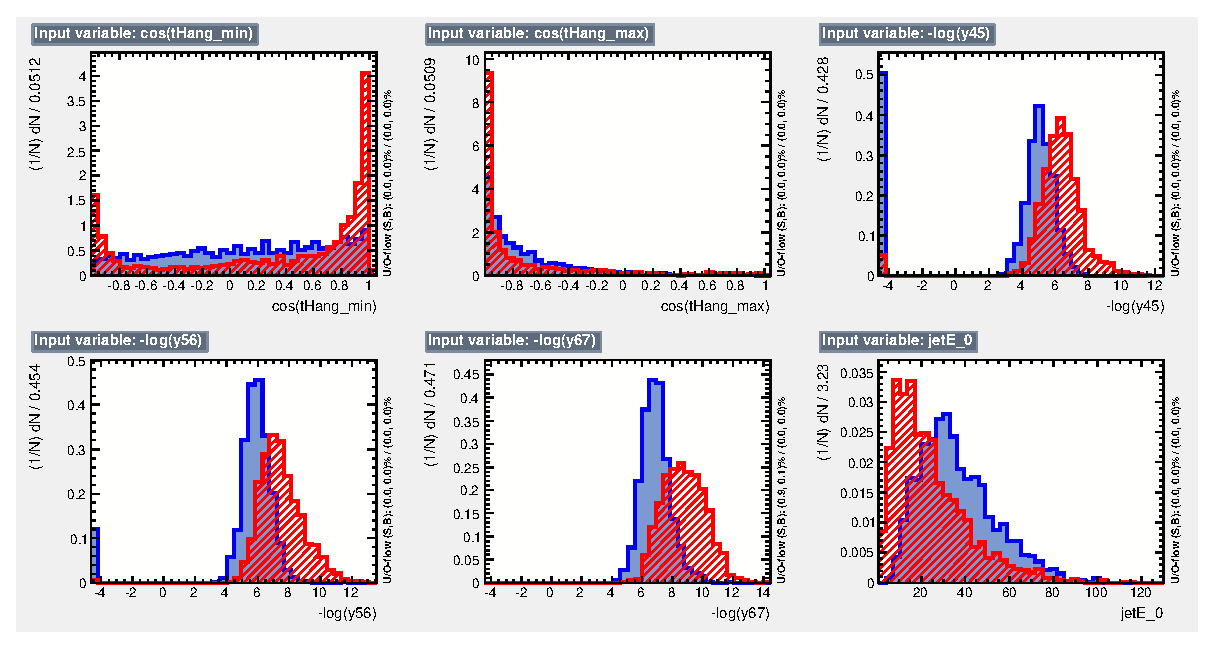
\includegraphics[width=0.95\textwidth]{../Pictures/Analysis/BDTs/variables_id_c4.eps}
	\caption{Input variables for the BDTs: [cos]; [cos]; [log]; [log]; [log]; lowest jet energy}
	\label{figure:analysis/results/tmva-inputs-4}
\end{figure}

\begin{figure}[h]
	\centering
	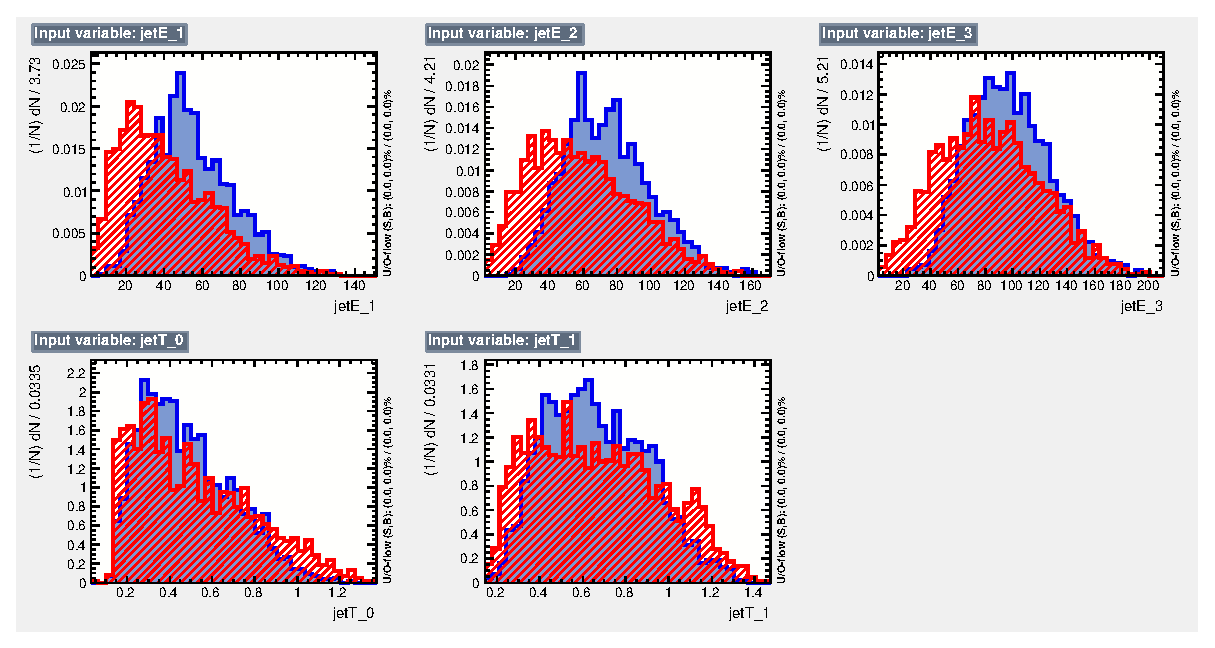
\includegraphics[width=0.95\textwidth]{../Pictures/Analysis/BDTs/variables_id_c5.eps}
	\caption{Input variables for the BDTs: second, third, and fourth lowest jet energies; [jetT_0]; [jetT_1]}
	\label{figure:analysis/results/tmva-inputs-5}
\end{figure}


%		%		%		%		%		%		%		%		%		%		%		%		%		%		%
%\section{Determination of sensitivity to CP-violation}
%[...]

%Another important avenue to pursue is \acrshort{CP}-violation in the Higgs sector. Since Higgs physics is still an emerging field, it is not yet known whether \acrshort{CP}-violation is present in the Higgs sector to the degree that the \acrlong{SM} predicts. It is also a fertile area for investigation of \acrshort{BSM} physics, as many \acrshort{BSM} models predict additional Higgs bosons, or Higgs bosons with characteristics that differ from the \acrshort{SM} Higgs.

%The $e^+ e^- \rightarrow t\overline{t}h$ event (see Fig. \ref{figure:physics/SM/feynman-tth}) is one process that is both accessible to \acrshort{CLIC}'s design energy and extremely useful for interrogating the Higgs sector for \acrshort{CP}-violation and \acrshort{BSM} physics. The production of Higgs bosons allows for several observables that would be sensitive to any Higgs bosons with an odd \acrshort{CP} quantum number (or ``CP-odd'' Higgs bosons). Determining the detectors' sensitivity to the ratio of \acrshort{CP}-odd and \acrshort{CP}-even Higgs bosons (also called the \acrshort{CP} mixing angle) will allow further understanding of the limits of the Standard Model, as well as the limits on the various \acrshort{BSM} physics models, and regions of interest for possible new physics.


%\subsection{CP-sensitive observables}
%[...]

%\subsubsection{Up-down asymmetry}
%The up-down asymmetry is a conceptually simple observable that has already been identified for investigating \acrshort{CP}-violation in the tth process. It is found by defining a plane from the vectors of the incoming electron and produced antitop, then finding the ratio of top quarks that are emitted above and below this plane (see Fig. \ref{figure:physics/SM/up-down}). If there is no \acrshort{CP}-violation in this process, the ratio will be even.
%
%Using the up-down asymmetry as an observable requires that the $W^+$ and $W^-$ can be distinguished from each other, and has thus far only been used for the semi-leptonic decay channel. In this case, the lepton produced by the decay of one of the W bosons identifies its charge, and thus the charge of the top quark that it has decayed from. While this method was not previously possible in the fully hadronic case, a method for applying it by using jet charge determination is discussed in Section \ref{section:physics/CP/jetcharge}.
%
%\begin{figure}
%	\centering
%	\begin{tikzpicture}[line width=1.3 pt,scale=1.8]
%	
%		\coordinate (origin) at (0,0) ;
%		\coordinate (electron) at (-3.5,0) ;
%		\coordinate (projection) at (2.5,0) ;
%		\coordinate (top) at (1,2) ;
%		\coordinate (antitop) at (3,-1) ;
%
%		\filldraw[fill=gray!5] (-2,0.75) -- (3,0.75) -- (2,-0.75) -- (-3,-0.75) -- cycle ;
%
%		\draw[fermion] (electron) -- (origin) ;
%		\draw[dashed] (origin) -- (2.5,0) ;
%		
%		\draw[fermionbar] (origin) -- (antitop) ;
%		\draw[fermion] (origin) -- (top) ;
%		
%		\draw pic[draw, -, "$\theta$", angle radius = 1cm] {angle = antitop--origin--top} ;
%		\draw[dotted] pic[draw, -, "$\phi$", angle radius = 2.5cm] {angle = antitop--origin--projection} ;
%		
%		\node at (-3.65,0.05) {$e^-$};
%		\node at (3.1,-1) {$\overline{t}$};
%		\node at (1.05,2.15) {$t$};
%	\end{tikzpicture}
%	\caption{Geometric diagram of the up-down asymmetry in tth events. The paths of the electron and antitop quark, and the angle $\phi$ between them define a plane. ``Up-going'' top quarks go above the plane, ``down-going'' top quarks go below.}
%	\label{figure:physics/SM/up-down}
%\end{figure}
%
%\subsubsection{[other ones]}
%[...]
%
%\subsection{Jet charge determination} \label{section:physics/CP/jetcharge}
%Previous analyses that have utilised the up-down asymmetry as an observable have focused exclusively on the semi-leptonic decay channel of tth events, as the presence of a lepton emitted by the top or antitop quark offers a simple and statistically robust method to distinguish between the two top quarks. In the hadronic decay channel each top emits a jet, and even in the ideal case where each particle resulting from the jet can be accurately reconstructed, the net charge will \emph{still} be an integer, since no particles with a non-integer charge can result from these decays.
%
%However, techniques developed in recent years, intended primarily for observations in \acrshort{ATLAS} at the \acrshort{LHC}, have refined methods for this, and using the work of [reference], it is now possible to obtain the total net charge of the jet -- that is, the charge of the initial quark that creates the jet. 
%
%This technique is strongly-dependent upon the accuracy and efficiency of both particle reconstruction and jet clustering, but these techniques are constantly improving, and \acrfull{PandoraPFA} and new jet clustering methods are becoming increasingly sophisticated. Combined with the cleaner final states in a lepton collider, these techniques allow the charge of a jet to be determined with useful confidence.
%
%The charge of a jet can be determined by summing the charges of all particles in the jet, weighted by $p_T$ and normalised by the $p_T$ of the entire jet:
%		
%\begin{displaymath}
%	\mathcal{Q}_\kappa^i = \frac{1}{(p_T^{jet})^\kappa} \sum_{j \in jet} Q_j (p_T^j)^\kappa
%\end{displaymath}
%
%Where $\kappa$ is some parameter between 0 and 1, typically set to 1. With this technique, it is possible to determine between quarks with charges of $+1/3e$, $-1/3e$, $+2/3e$, and $-2/3e$ with [some level of confidence].
%
%\subsubsection{Jet clustering algorithms}
%Since this method relies upon jets it is strongly dependent upon jet reconstruction, and thus on the choice of jet clustering algorithm and parameters. Previous analyses of tth events have used a two-step reclustering approach, using the $k_t$ algorithm for the initial clustering and the Durham algorithm for reclustering. These algorithms were chosen as the relative difference between the jet shapes is more important than their absolute shapes, so other algorithms do not provide any benefits.
%
%The Valencia algorithm, however, gives improved performance in the cleaner final states of a lepton collider, for which it was especially designed, and many analyses are now transitioning to using the Valencia algorithm.